\chapter{Planejamento}
Conforme descrito no Capítulo \ref{cap:introducao}, este trabalho será constituído de cinco etapas.
Em um primeiro momento, a etapa de diagnóstico foi realizada e os sistemas relacionados e suas funcionalidades em comum foram apresentadas no Capítulo \ref{cap:sistemas_relacionados}. Em seguida, o objetivos do trabalho foram definidos. 

Para alcançar os objetivos propostos foi feita uma avaliação do escopo da plataforma Empurrando Juntos, que é foco de contribuição deste trabalho.
Nessa avaliação foram mapeadas as entidades principais, seus atributos e os relacionamentos entre elas. Esse mapeamento pode ser visto na Figura \ref{fig:entidades}.

\begin{figure}[h!]
\centering
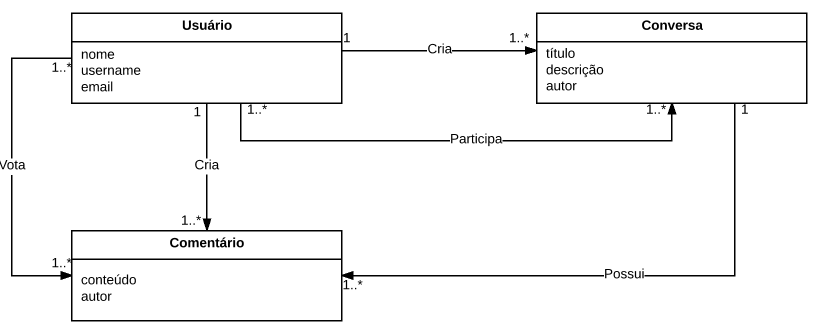
\includegraphics[scale=0.5]{figuras/entidades.png}
\caption{Entidades da API}
\label{fig:entidades}
\end{figure}


A API a ser criada faz parte de uma estrutura que será denominada como Pentano. O Pentano é constituído por dois módulos: o \textit{server}, que é o módulo da API
e o \textit{Math} que é o módulo responsável pela clusterização. Essa estrutura pode ser melhor visualizada na Figura \ref{fig:pentano}.


\begin{figure}[h!]
\centering
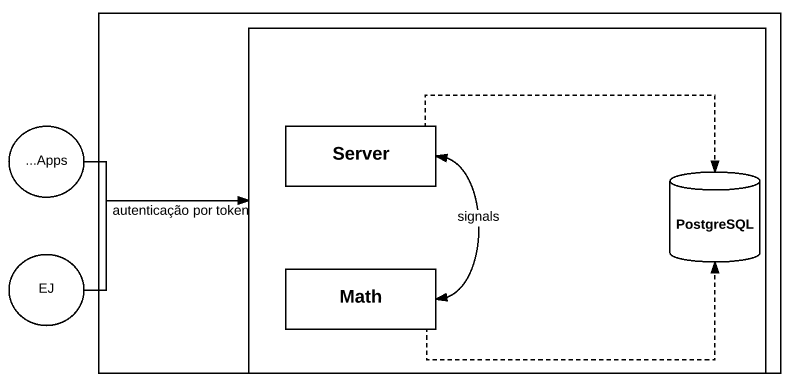
\includegraphics[scale=0.5]{figuras/esquema_pentano.png}
\caption{Estrutura do Pentano}
\label{fig:pentano}
\end{figure}